\subsection{Parametrization of Datapoints}
\label{ssec:parametrization}
In addition to the reconstructed surface we need the following information for the least squares fit: 
\begin{itemize}
\item Which \ac{NURBS}-patch does each datapoint of the reconstructed surface belong to?
\item What are the values of $u,v$ parameters of the datapoint on the patch?
\end{itemize}
\subsubsection{Two-scale Dual Contouring}
Before we can distribute datapoints to \ac{NURBS}-patches, we first have to find out how these patches look like. Since we want to have as few patches as possible we do not simply turn every \ac{quad} from the surface reconstruction into a patch. Instead  we try to find a surface with as few \acp{quad} as possible, while keeping the same topology as our initially reconstructed surface. This coarse surface will be assumed to be the patch distribution for the later steps.


Therefore, in our algorithm we are reconstructing the surface on two different scales: a coarse and a fine scale. The coarse scale data is deduced from the fine scale data by recursively applying the following algorithm:
\begin{enumerate}
\item Combine sets of eight connected voxels with egde-length $a$ into a coarse voxel with edgelength $2a$ (see \autoref{sfig:coarsenA}).
\item Decide whether the new voxel resembles an inner ($=1$) or outer ($=0$) voxel. This is done by taking the mean value of the contributing eight voxels. If the mean value is above a certain threshold $t$, the new voxel is considered as an inner voxel. We picked $t=\frac{1}{8}$, i.e. if at least two voxels out of eight are inner voxels, the resulting voxel is considered being an inner voxel.
\item For the resolution of non-manifold edges, additional coarse voxel grids are generated. These grids are shifted by edge-length $a$ (see \autoref{sfig:coarsenB}).
\end{enumerate}
\begin{figure}
\begin{subfigure}{.45\textwidth}
\begin{center}
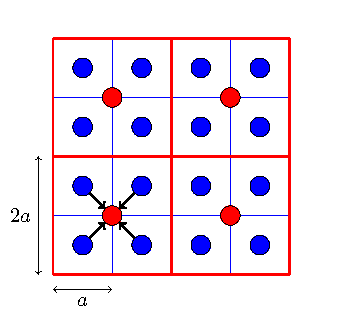
\includegraphics[scale=1]{Pictures/tikzCoarsen/coarsen.pdf}
\end{center}
\subcaption{Sets of 8 (4 in 2D) fine voxels (blue) are recursively combined to form one coarse voxel (red).}
\label{sfig:coarsenA}
\end{subfigure}\hfill
\begin{subfigure}{.45\textwidth}
\begin{center}
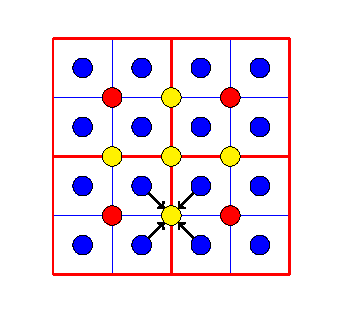
\includegraphics[scale=1]{Pictures/tikzCoarsen/coarsenMani.pdf}
\end{center}
\subcaption{Addition voxels (yellow) are introduced in a non-aligned grid for non-manifold resolution on the coarse scale.}
\label{sfig:coarsenB}
\end{subfigure}
\caption{Coarsening scheme applied in \emph{Two-scale \acl{DC}}.}
\label{fig:coarsen}
\end{figure}
One iteration of this coarsening scheme is referred to as one \emph{coarsening step}. Applying this scheme recursively allows higher coarsening and results in multiple coarsening steps.

Here, we apply \ac{DC} to both datasets and obtain two different reconstructed surfaces.
The coarse scale surface is used as a patch distribution and from the fine scale we obtain our datapoints. The \ac{NURBS} will be fitted to these datapoints. We call this approach \emph{Two-scale \acl{DC}} (see \autoref{fig:TwoScale}).
Of course this simple approach comes with drawbacks:
\begin{itemize}
\item We cannot guarantee that the coarse and the fine scale have exactly the same topology. Topological details of the fine scale, which do not exist on the coarse scale, are lost.
\item Both resolutions have to be chosen manually, since we do not have a criterion for evaluating the quality of the coarse scale surface reconstruction.
\end{itemize}
These drawbacks are especially bad for complex surfaces -- like the output of topology optimization -- where the topological details mentioned above are not an exception, but the default case. There are more elaborate surface extraction schemes that handle these problems. For the interested reader, alternative schemes such as \emph{Dual Marching Cubes} \cite{ScottSchaefer2004} or \emph{Manifold Dual Contouring} \cite{Schaefer2007}, are included in \autoref{appx:AltSurfRecon}.
\subsubsection{Projection of Datapoints onto Quads}
Now that we have constructed a \ac{NURBS}-patch distribution, we can estimate the parametrization of the datapoints on the fine scale by projecting them onto the patches: 

For this procedure we do the following steps:

\begin{enumerate}
\item Find out onto which of these patches a datapoint should be projected. This can be done by simply measuring the distance from the datapoint to the centroid of each patch and deciding to project onto the patch with the smallest distance.
\item Project the point onto the target patch. For this, we want the whole \ac{quad} to be parametrized on $\left(u,v\right)\in\left[0,1\right]^2$. This is done by first approximating the quad (which may not necessarily be planar) with its least squares fit plane. Then a projection onto this plane is done by applying a simple basis transformation\footnote{This basis transformation is computed in a very efficient way by computing the QR-decomposition for the basis of each patch only once and applying it to each datapoint projected onto this patch.}.
\end{enumerate}

The projection might lead to parameters $\left(u,v\right)\not\in\left[0,1\right]^2$ for some of the datapoints. As we only produce surfaces for $\left(u,v\right)\in\left[0,1\right]^2$, these are then not on the surface. If we still include them in the fitting, these will then influence parts of the surface that are not there, leading to unwanted fitting behaviour such as wiggles and turns. 

We have tried several methods to solve this problem. For example, one might consider scaling the parameter space of each quad to $\left[0,1\right]^2$, which however leads to inconsistencies in parameter assignemt between neighbouring quads with different scaling. Another solution, cropping the parameter domain by shifting all parameters outside $\left[0,1\right]^2$ to the closest border (i.e. for $u \text{ or } v < 0$ is assigned to $0$, $u \text{ or } v >1$ is assigned to $1$), also leads to problems, as points in different regions of space then can end up having the same parameter values. To simplify the treatment, we therefore currently only consider the points parametrized inside $\left[0,1\right]^2$, and omit all points outside from this step onwards. \tododone[author=Erik]{Benni{@}Erik: Whaaaaaat?,{@}Benni: Works? }.

After completing all these steps we obtain the following data for the subsequent steps of our algorithm:
\begin{itemize}
\item a coarse surface delivering the topology for our \ac{NURBS}-patches in Peters' Scheme
\item a set of datapoints from the fine scale with coordinates $\left(x,y,z\right)^T\in\mathbb{R}^3$ and parameters $\left(u,v\right)\in\left[0,1\right]^2$, where each datapoint is associated with a \ac{NURBS}-patch. 
\end{itemize}
For a sample output of our algorithm for a 2D case, see \autoref{fig:TwoScale}.

\begin{figure}
\begin{center}
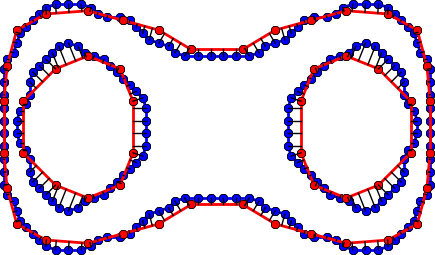
\includegraphics[width=.5 \textwidth]{Pictures/SurfaceReconstruction/TwoScale}
\caption{Twoscale \acl{DC} with a coarse surface reconstruction (red) and a fine one (blue). The datapoints from the fine scale are projected onto the edges from the coarse scale (black lines).}
\label{fig:TwoScale}
\end{center}
\end{figure}
\begin{comment}
\subsubsection{Parameter estimation}
\todo[inline]{explain different strategies, comparison of final results would be great (could also be part of third milestone?)}
\todo[inline]{show possible problems}
\end{comment}
